\chapter{Grundlagen}

In diesem Kapitel wird eine kurze Einführung in die Grundlagen von Unterteilungsalgorithmen gegeben.

\section{Unterteilungsalgorithmen}

Unterteilungsalgorithmen erzeugen aus einem Ausgangspolygonnetz eine glatte Fläche.
Die glatte Zielfläche ist dabei der Grenzwert eines unendlichen, rekursiven Verfeinerungsschemas.
\autoref{fig:sd} visualisiert die Anwendung eines Unterteilungsalgorithmus auf eine Kurve und auf eine Fläche.
Nach mehrfacher Anwendung der Unterteilung konvergiert die Kurve oder Fläche gegen die glatte Zielkurve bzw. Zielfläche.

\begin{figure}
  \centering
  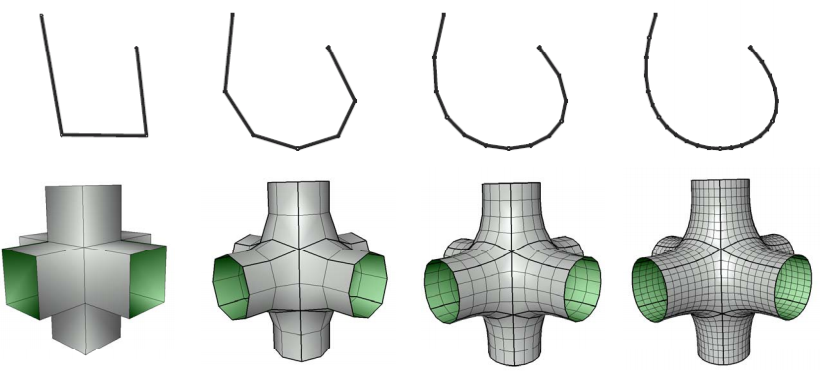
\includegraphics[width=0.8\textwidth]{content/media/sd.png}
  \caption{Unterteilungsalgorithmus - Kurve und Fläche \cite{Standford.24.07.2015}}
  \label{fig:sd}
\end{figure}

Unterteilungsalgorithmen kann man anhand ihrer Eigenschaften kategorisieren.
Ein Unterscheidungskriterium betrifft die Art und Weiße, wie unterteilt wird.
Man unterscheidet dabei zwischen \emph{primal} und \emph{dual}.

\begin{description}
 \item[Primal] Bei dieser Strategie wird die Oberfläche unterteilt (\enquote{face split}).
\autoref{fig:sd_primal} stellt diese Methode für ein Dreicksnetz und ein Vierecksnetz dar.
 \item[Dual] Auf der anderen Seite ist es möglich Eckpunkte in mehrere Eckpunkte aufzusplitten (\enquote{vertex split}).
 Diese Methode ist in \autoref{fig:sd_dual} abgebildet.

\end{description}
\begin{figure}
  \centering
  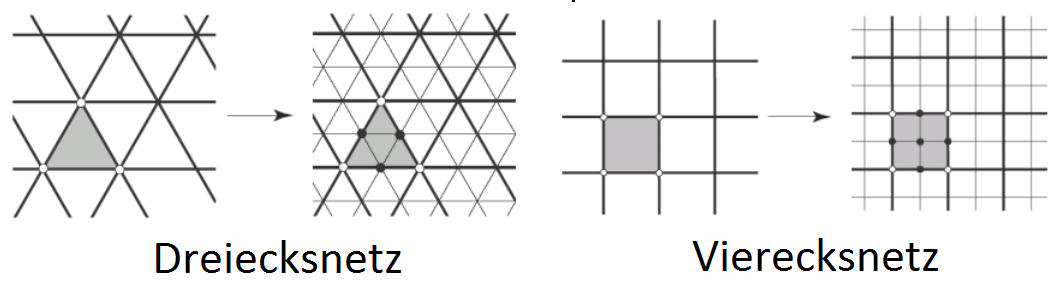
\includegraphics[width=0.7\textwidth]{content/media/sd_primal}
  \caption{Primal (face split) \cite{Standford.24.07.2015}}
  \label{fig:sd_primal}
\end{figure}

\begin{figure}
  \centering
  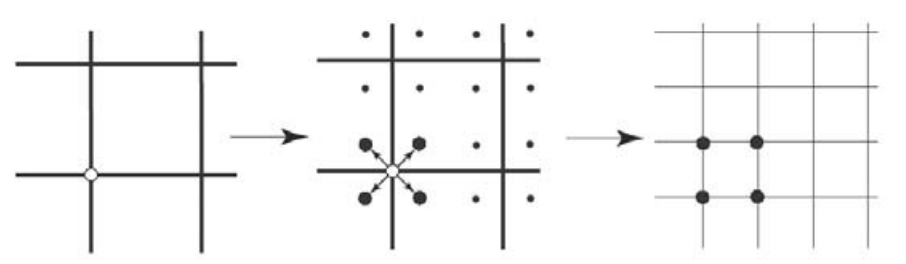
\includegraphics[width=0.7\textwidth]{content/media/sd_dual}
  \caption{Dual (vertex split) \cite{Standford.24.07.2015}}
  \label{fig:sd_dual}
\end{figure}

Ein weiteres wesentliches Merkmal ist, ob Kontrollpunkte interpoliert werden oder nicht. 
\begin{description}
 \item[Approximation] Kontrollpunkte werden nicht interpoliert.
 \item[Interpolation] Kontrollpunkte werden interpoliert.
\end{description}

\autoref{tab:sd_comp_primal} und \autoref{tab:sd_comp_dual} listet die bekanntesten Unterteilungsalgorithmen auf und ordnet diese den Kategorien zu.
Zu jedem Algorithmus ist zusätzlich die \enquote{Glattheit} der Oberfläche angegeben (C-Stetigkeit).
Die Unterteilungsalgorithmen erzeugen auf beliebig angeordnete Netze \(C^1\) stetige Flächen.
In den \autoref{tab:sd_comp_primal} und \autoref{tab:sd_comp_dual} wird die Stetigkeit für den
\emph{regulären} Fall angegeben.
Die C-Stetigkeit kann auch als Maß über die Qualität des Unterteilungsalgorithmus fungieren.
\begin{table}
\center
\caption{Unterteilungsalgorithmen Übersicht primal \cite[S. 65]{Zorin.subdivcourse}}
\label{tab:sd_comp_primal}
\begin{tabular}{l|c|c|}
& \multicolumn{2}{c|}{\textbf{Primal}}\\
\hline
& \textbf{Dreiecksnetz} & \textbf{Vierecksnetz}\\
\hline
\textbf{Approximation} & Loop \((C^2)\) & Catmull-Clark \((C^2)\)\\
\textbf{Interpolation} & Butterfly \((C^1)\) & Kobbelt \((C^1)\)\\
\end{tabular}
\end{table}
\begin{table}
\center
\caption{Unterteilungsalgorithmen Übersicht dual \cite[S. 65]{Zorin.subdivcourse}}
\label{tab:sd_comp_dual}
\begin{tabular}{c}
\\
\hline
\textbf{Dual}\\
\hline
Doo-Sabin \((C^1)\) \\
Biquartic \((C^2)\) \\
\end{tabular}
\end{table}
\autoref{fig:sd_comp} vergleicht die vier unterschiedlichen Unterteilungsalgorithmen Catmull-Clark, Loop, Doo-Sabin und Butterfly.
Man erkennt deutlich den interpolierenden Unterteilungsalgorithmus (Butterfly),
da dieser durch die harten Interpolationsbedingungen im Vergleich zu den approximierenden Algorithmen viel \enquote{welliger} ist. \cite{Zorin.subdivcourse}
\begin{figure}
  \centering
  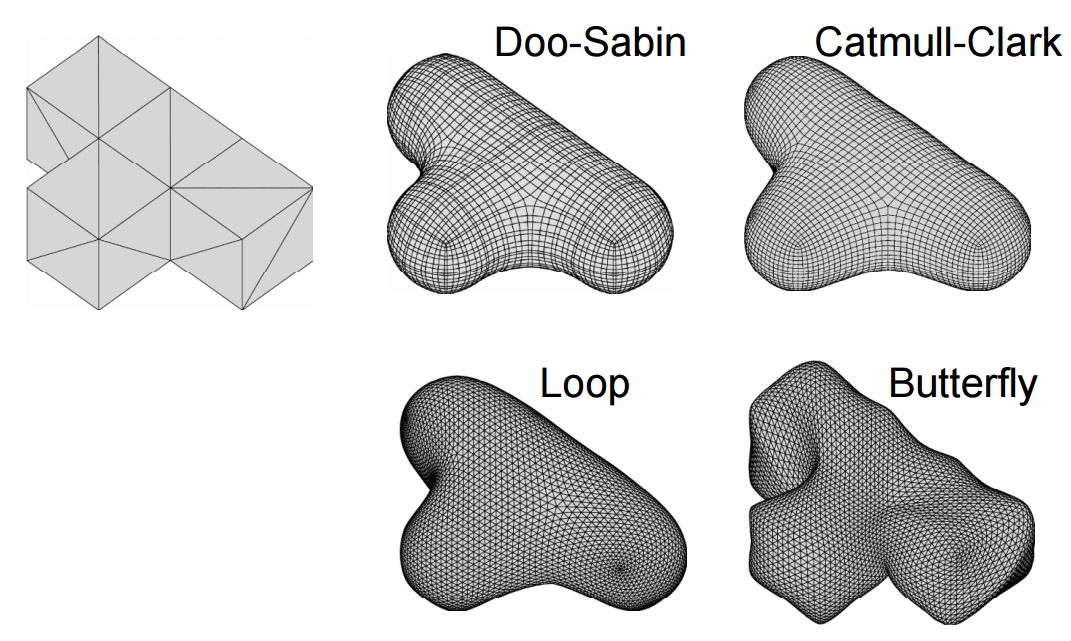
\includegraphics[width=0.9\textwidth]{content/media/sd_overview.png}
  \caption{Vergleich der Unterteilungsalgorithmen \cite{Standford.24.07.2015}}
  \label{fig:sd_comp}
\end{figure}

\section{Auswahl von Unterteilungsalgorithmen}

Für das Projekt sollen folgende Algorithmen implementiert werden:
\begin{itemize}
	\item Catmull-Clark
	\item Loop
	\item Doo-Sabin
	\item Butterfly
\end{itemize}
Dies sind die wichtigsten Vertreter für Dreiecks- und Vierecksnetze.
Prinzipiell sind jedoch noch weitere Algorithmen denkbar.
\cite[S. 65ff]{Zorin.subdivcourse} \cite{Standford.24.07.2015}

\section{Catmull-Clark}

\subsection{Allgemein}

Der Catmull-Clark Algorithmus wurde 1978 von Edwin Catmull und James Clark entwickelt.
Er basiert auf bi-cubic uniform B-spline surfaces.
Der ursprüngliche Algorithmus war nur für Vierecksnetze definiert.
Hier wird eine erweiterte Form verwendet, die mit beliebiger Topologie umgehen kann.
Das neu erzeugte Netz ist immer ein Vierecksnetz.
Jedes n-Gon im Eingabenetz wird in n Quads
im Ausgabenetz umgewandelt.
Die Kontrollpunkte des Netzes werden durch Unterteilung approximiert.
Catmull-Clark erzeugt im Normalfall \(C^2\) Flächen,
an extraordinären Stellen mit Valence ungleich vier jedoch
nur \(C^1\).
\cite[S. 75ff]{Zorin.subdivcourse} \cite[S. 52ff]{Standford.24.07.2015}


\subsection{Unterteilungsregel}

Um ein Kontrollnetz nach Catmull-Clark zu unterteilen sind vier Schritte notwendig.
\begin{enumerate}
	\item Füge für jedes Polygon einen neuen Punkt hinzu (face point).
	\item Füge für jede Kante einen neuen Punkt hinzu (edge point).
	\item Berechne für jeden alten Kontrollpunkt die neue Position (original point).
	\item Verbinde die Punkte (face point, edge point, original point), sodass diese ein
	neues verfeinerten Netz erzeugen (face split).
\end{enumerate}

\autoref{fig:sd_catmull_mask} zeigt die Masken, mit denen die jeweiligen Punkte für ein Viereck berechnet werden können.
Im folgenden wird der allgemeinere Fall für beliebige Polygone beschrieben.
\begin{figure}
\centering
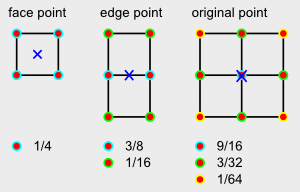
\includegraphics[width=0.5\textwidth]{content/media/sd_catmull_mask.png}
\caption{Catmull-Clark Maske für ein Viereck \cite{yoshihitoyagi.23.12.2015}}
\label{fig:sd_catmull_mask}
\end{figure}

\subsubsection*{Face Point}
Der face point berechnet sich als Mittelwert der Kontrollpunkte des Polygons.
Bei einem Viereck wie in \autoref{fig:sd_catmull_mask} hat somit jeder Kontrollpunkt
ein Gewicht von 1/4.

\subsubsection*{Edge Point}
Der edge point wird von den anliegenden Polygone beeinflusst.
Dieser errechnet sich aus dem Durchschnitt der zwei benachbarten Face Points und den
beiden Kontrollpunkten der Kante.

\subsubsection*{Original Point}
Jeder original point wird aktualisiert.
Die Berechnung wird folgendermaßen durchgeführt:\\
\(
new\_point=(Q/n) + (2R/n) + (S*(n-3)/n)\\
n:\ Valence\\
Q:\ Durchschnitt\ der\ umliegenden\ face\ points\\
R:\ Durchscnitt\ aller\ umliegenden\ Mittelpunkte\ der\ Ecken\ (!=\ edge\ point)\\
S:\ priginal\ point
\)

\subsubsection*{Face Split}
Nun sind alle notwendigen Punkte berechnet.
Die Punkte müssen durch Kanten zu gültigen Quads zusammengesetz werden.
Ein Quad besteht aus den vier Ecken:
\begin{itemize}
 \item Original Point
 \item Edge Point 1
 \item Face Point
 \item Edge Point 2
\end{itemize}
Für jedes Polygon mit n Ecken entstehen n Quads.
\autoref{fig:sd_catmull_split} zeigt das Schema für ein Viereck.
\begin{figure}
\centering
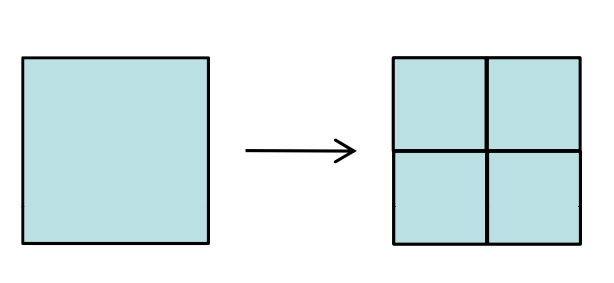
\includegraphics[width=0.3\textwidth]{content/media/sd_catmull_split.png}
\caption{Catmull-Clark face split \cite[S. 52f]{Standford.24.07.2015}}
\label{fig:sd_catmull_split}
\end{figure}
\cite{rosettacode.23.12.2015}
\cite{rorydriscoll.23.12.2015}
\cite{yoshihitoyagi.23.12.2015}

\subsection{Randregel}

Für Ränder (boundary cases) können die Koeffizienten für kubische Splines verwendet werden.
Diese führen zu akzeptablen Ergebnissen, garantieren formal jedoch keine \(C^1\) Stetigkeit mehr. \cite[S. 75f]{Zorin.subdivcourse}
\autoref{fig:sd_catmull_boundary} zeigt die Gewichtung für Ränder.
Der edge point wird durch den Mittelwert der Ecken berechnet.
Um den neuen original point zu berechnen, wird die rechte Maske aus \autoref{fig:sd_catmull_boundary}
verwendet.

\begin{figure}
\centering
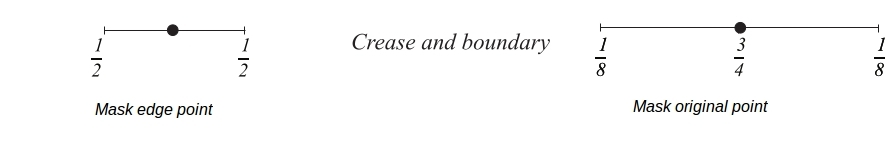
\includegraphics[width=1.0\textwidth]{content/media/sd_catmull_boundary.jpg}
\caption{Catmull-Clark Crease/Boundary \cite[S. 76]{Zorin.subdivcourse}}
\label{fig:sd_catmull_boundary}
\end{figure}




\section{Loop} \label{sec:loop}

\subsection{Allgemein}

Charles Loop hat 1987 einen Unterteilungsalgorithmus für Dreiecksnetze entwickelt.
Der Loop Algorithmus basiert auf quartischen Box Splines und approximiert die Kontrollpunkte.
An extraordinären Stellen mit Valenz ungleich sechs erzeugt Loop \(C^1\) stetige Flächen,
im regulären Fall \(C^2\).
\cite[S. 70f]{Zorin.subdivcourse} \cite[S. 56f]{Standford.24.07.2015}

\subsection{Unterteilungs- und Randregeln}

Die Unterteilung erfolgt in drei Schritten.
\begin{enumerate}
\item Berechne für jede Kante einen Edge Point. Dieser wird auch als Odd Vertex bezeichnet.
\item Berechne für jeden Vertex eine neue Position. Dieser wird auch als Even Vertex bezeichnet.
\item Ersetze jedes Dreieck durch vier neue Dreiecke.
\end{enumerate}

\autoref{fig:sd_loop_mask} zeigt die Masken für die Unterteilung
und für Randfälle.
Entlang des Randes (boundary/crease) wird eine kubische Spline Kurve erzeugt.
\cite[S. 70]{Zorin.subdivcourse}
\begin{figure}
\centering
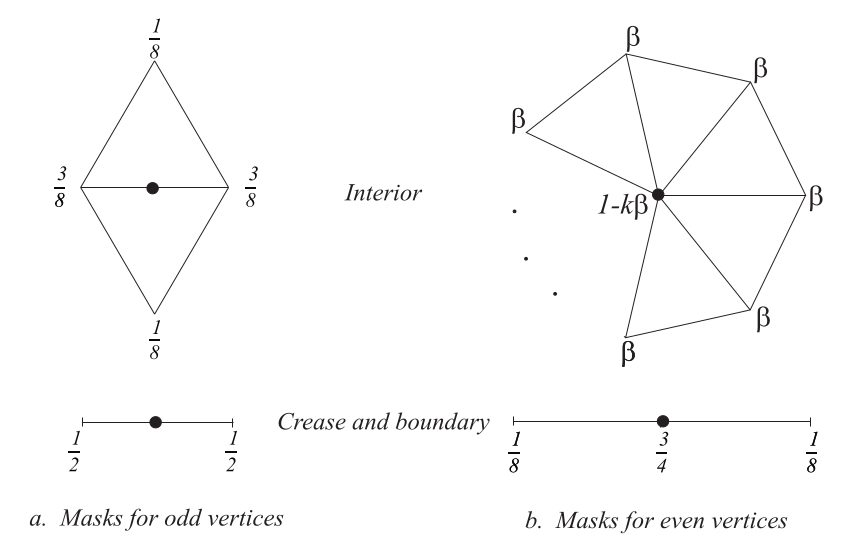
\includegraphics[width=1.0\textwidth]{content/media/sd_loop_mask.jpg}
\caption{Loop Maske \cite[S. 70f]{Zorin.subdivcourse}}
\label{fig:sd_loop_mask}
\end{figure}

\subsubsection*{Odd Vertex}
Die Odd Vertices werden nach der linken Maske aus \autoref{fig:sd_loop_mask} berechnet.
Für Ränder wird der Mittelwert genommen.

\subsubsection*{Even Vertex}

Bei Even Vertices muss für die Berechnung ein Faktor \(\beta\) bestimmt werden.
\autoref{fig:sd_loop_mask} veranschaulicht die Struktur.
Ist \(\beta\) bekannt, kann der Vertex wie folgt berechnet werden:\\
\(
even\_vertex = old\_vertex * (1 - k * beta) + (sum\_of\_surrounding\_vertices) * beta\\
k:\ Valenz
\)
\\
Für die Bestimmung von \(\beta\) gibt es mehrere Möglichkeiten:
\begin{description}
\item[Original nach Loop]  \(\beta=\frac{1}{k}(\frac{5}{8}-(\frac{3}{8}+\frac{1}{4}cos(\frac{2\pi}{k}))^2)\)
\item[Variation nach Warren] \mbox{}
	\begin{itemize}
		\item für \(k > 3, \beta = \frac{3}{8k}\)
		\item für \(k = 3, \beta = \frac{3}{16}\)	
	\end{itemize}
\end{description}
Die Variation nach Warran hat den Vorteil, dass diese einfacher berechnet werden kann
und somit eine perfomantere Implementierung möglich ist.
Die Variante nach Warren ist auch in Subvis implementiert.

Für Ränder muss \(\beta\) nicht bestimmt werden.
Hier kann das einfache Schema aus \autoref{fig:sd_loop_mask} angewendet werden.
\cite{Carnegie}
\cite{Standford.Loop}
\cite[S. 70f]{Zorin.subdivcourse}

\subsubsection*{Face Split}

Jedes Dreieck wird schließlich, wie in \autoref{fig:sd_loop_split} gezeigt, in vier neue Dreiecke aufgeteilt.

\begin{figure}
\centering
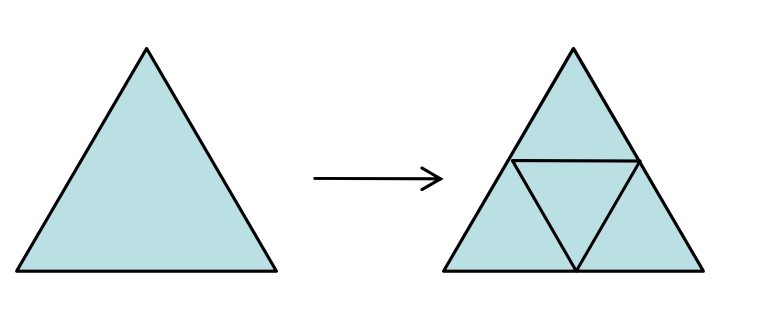
\includegraphics[width=0.3\textwidth]{content/media/sd_loop_split.png}
\caption{Loop Face Split \cite[S. 56f]{Standford.24.07.2015}}
\label{fig:sd_loop_split}
\end{figure}


\section{Doo Sabin}
\section{Butterfly} \label{sec:butterfly}

\subsection{Allgemein}

Der Butterfly Algorithmus ist ein interpolierender Unterteilungsalgorithmus,
der von Nira Dyn, David Levine und John A. Gregory entwickelt wurde.
Butterfly arbeitet auf Dreiecksnetzen und erzeugt an regulären Stellen
\(C^1\) stetige Flächen, an extraordinären Stellen
(Valenz gleich drei oder größer sieben) jedoch lediglich \(C^0\).
\cite[S. 64ff]{Standford.24.07.2015} \cite[S. 72ff]{Zorin.subdivcourse}
\cite{Seeger01asub-atomic}
\cite{Gamasutra}
\cite{Sharp}
\cite{Zorin:1996:ISM:237170.237254}

\subsection{Unterteilungs- und Randregeln}

Der Algorithmus besteht aus zwei Schritten:
\begin{enumerate}
\item Berechne für jede Kante einen Edge Point.
\item Ersetze jedes Dreieck durch vier neue Dreiecke.
\end{enumerate}

\begin{figure}
\centering
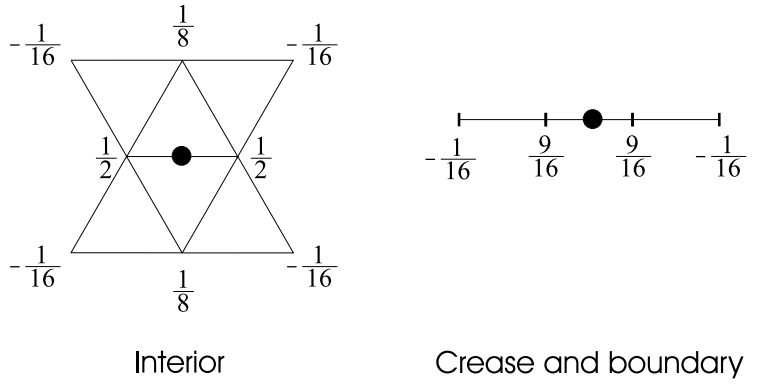
\includegraphics[width=0.8\textwidth]{content/media/sd_butterfly_mask.jpg}
\caption{Butterfly Eight-Point Stencil und Randregel \cite{Seeger01asub-atomic}}
\label{fig:sd_butterfly_mask}
\end{figure}

\subsubsection*{Edge Point}
Die Berechnung des Edge Points wird mit dem sogenannten Eight-Point Stencil
aus \autoref{fig:sd_butterfly_mask} durchgeführt.
Die Regel für den Randfall ist daneben abgebildet.


Da die Punkte beim Butterfly interpoliert werden, müssen die alten Vertices
(wie bisher bei approximierenden Algorithmen) nicht neu berechnet werden. 

\subsubsection*{Face Split}
Der Face Split ist identisch zum Loop Face Split.
Jedes Dreieck wird in vier neue Dreiecke aufgeteilt (\autoref{fig:sd_loop_split}).
\cite[S. 64ff]{Standford.24.07.2015} \cite[S. 72ff]{Zorin.subdivcourse}
\cite{Seeger01asub-atomic}
\cite{Gamasutra}
\cite{Sharp}
\cite{Zorin:1996:ISM:237170.237254}
